\documentclass[twoside]{book}

% Packages required by doxygen
\usepackage{fixltx2e}
\usepackage{calc}
\usepackage{doxygen}
\usepackage[export]{adjustbox} % also loads graphicx
\usepackage{graphicx}
\usepackage[utf8]{inputenc}
\usepackage{makeidx}
\usepackage{multicol}
\usepackage{multirow}
\PassOptionsToPackage{warn}{textcomp}
\usepackage{textcomp}
\usepackage[nointegrals]{wasysym}
\usepackage[table]{xcolor}

% Font selection
\usepackage[T1]{fontenc}
\usepackage[scaled=.90]{helvet}
\usepackage{courier}
\usepackage{amssymb}
\usepackage{sectsty}
\renewcommand{\familydefault}{\sfdefault}
\allsectionsfont{%
  \fontseries{bc}\selectfont%
  \color{darkgray}%
}
\renewcommand{\DoxyLabelFont}{%
  \fontseries{bc}\selectfont%
  \color{darkgray}%
}
\newcommand{\+}{\discretionary{\mbox{\scriptsize$\hookleftarrow$}}{}{}}

% Page & text layout
\usepackage{geometry}
\geometry{%
  a4paper,%
  top=2.5cm,%
  bottom=2.5cm,%
  left=2.5cm,%
  right=2.5cm%
}
\tolerance=750
\hfuzz=15pt
\hbadness=750
\setlength{\emergencystretch}{15pt}
\setlength{\parindent}{0cm}
\setlength{\parskip}{3ex plus 2ex minus 2ex}
\makeatletter
\renewcommand{\paragraph}{%
  \@startsection{paragraph}{4}{0ex}{-1.0ex}{1.0ex}{%
    \normalfont\normalsize\bfseries\SS@parafont%
  }%
}
\renewcommand{\subparagraph}{%
  \@startsection{subparagraph}{5}{0ex}{-1.0ex}{1.0ex}{%
    \normalfont\normalsize\bfseries\SS@subparafont%
  }%
}
\makeatother

% Headers & footers
\usepackage{fancyhdr}
\pagestyle{fancyplain}
\fancyhead[LE]{\fancyplain{}{\bfseries\thepage}}
\fancyhead[CE]{\fancyplain{}{}}
\fancyhead[RE]{\fancyplain{}{\bfseries\leftmark}}
\fancyhead[LO]{\fancyplain{}{\bfseries\rightmark}}
\fancyhead[CO]{\fancyplain{}{}}
\fancyhead[RO]{\fancyplain{}{\bfseries\thepage}}
\fancyfoot[LE]{\fancyplain{}{}}
\fancyfoot[CE]{\fancyplain{}{}}
\fancyfoot[RE]{\fancyplain{}{\bfseries\scriptsize Generated by Doxygen }}
\fancyfoot[LO]{\fancyplain{}{\bfseries\scriptsize Generated by Doxygen }}
\fancyfoot[CO]{\fancyplain{}{}}
\fancyfoot[RO]{\fancyplain{}{}}
\renewcommand{\footrulewidth}{0.4pt}
\renewcommand{\chaptermark}[1]{%
  \markboth{#1}{}%
}
\renewcommand{\sectionmark}[1]{%
  \markright{\thesection\ #1}%
}

% Indices & bibliography
\usepackage{natbib}
\usepackage[titles]{tocloft}
\setcounter{tocdepth}{3}
\setcounter{secnumdepth}{5}
\makeindex

% Hyperlinks (required, but should be loaded last)
\usepackage{ifpdf}
\ifpdf
  \usepackage[pdftex,pagebackref=true]{hyperref}
\else
  \usepackage[ps2pdf,pagebackref=true]{hyperref}
\fi
\hypersetup{%
  colorlinks=true,%
  linkcolor=blue,%
  citecolor=blue,%
  unicode%
}

% Custom commands
\newcommand{\clearemptydoublepage}{%
  \newpage{\pagestyle{empty}\cleardoublepage}%
}

\usepackage{caption}
\captionsetup{labelsep=space,justification=centering,font={bf},singlelinecheck=off,skip=4pt,position=top}

%===== C O N T E N T S =====

\begin{document}

% Titlepage & ToC
\hypersetup{pageanchor=false,
             bookmarksnumbered=true,
             pdfencoding=unicode
            }
\pagenumbering{roman}
\begin{titlepage}
\vspace*{7cm}
\begin{center}%
{\Large My Project }\\
\vspace*{1cm}
{\large Generated by Doxygen 1.8.11}\\
\end{center}
\end{titlepage}
\clearemptydoublepage
\tableofcontents
\clearemptydoublepage
\pagenumbering{arabic}
\hypersetup{pageanchor=true}

%--- Begin generated contents ---
\chapter{File Index}
\section{File List}
Here is a list of all files with brief descriptions\+:\begin{DoxyCompactList}
\item\contentsline{section}{\hyperlink{Lab1_8c}{Lab1.\+c} }{\pageref{Lab1_8c}}{}
\end{DoxyCompactList}

\chapter{File Documentation}
\hypertarget{HiTester_8cpp}{}\section{Hi\+Tester.\+cpp File Reference}
\label{HiTester_8cpp}\index{Hi\+Tester.\+cpp@{Hi\+Tester.\+cpp}}
{\ttfamily \#include $<$iostream$>$}\\*
{\ttfamily \#include $<$vector$>$}\\*
{\ttfamily \#include $<$string$>$}\\*
Include dependency graph for Hi\+Tester.\+cpp\+:
\nopagebreak
\begin{figure}[H]
\begin{center}
\leavevmode
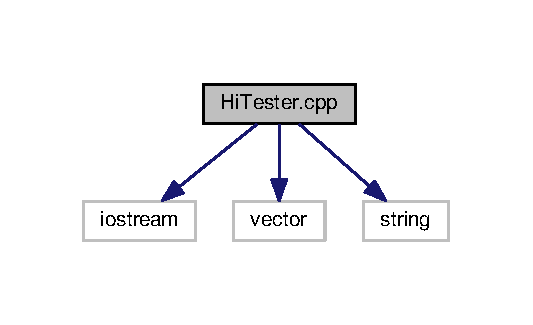
\includegraphics[width=256pt]{HiTester_8cpp__incl}
\end{center}
\end{figure}
\subsection*{Functions}
\begin{DoxyCompactItemize}
\item 
vector$<$ int $>$ \hyperlink{HiTester_8cpp_ab1aa54e6e8c6afe839f1b2e1456634b0}{add} (int\mbox{[}$\,$\mbox{]}, int\mbox{[}$\,$\mbox{]}, int len1, int len2)
\item 
bool \hyperlink{HiTester_8cpp_a50e1d1eacaf36a74c01e52a2d1dd9ecd}{check} (vector$<$ int $>$ v)
\item 
bool \hyperlink{HiTester_8cpp_ade6e4a501f91be609ebec2ff4f53f177}{equal\+To} (vector$<$ int $>$ v1, vector$<$ int $>$ v2)
\item 
bool \hyperlink{HiTester_8cpp_a4c5b23015a428515b186958f049fa9ff}{not\+Equal} (vector$<$ int $>$ v1, vector$<$ int $>$ v2)
\item 
bool \hyperlink{HiTester_8cpp_a9a5f44b0a0b7a897f035c1137b066e16}{greater\+Than\+Or\+Equal} (vector$<$ int $>$ v1, vector$<$ int $>$ v2)
\item 
bool \hyperlink{HiTester_8cpp_a39022c885b9928f13a6c4987dc563b60}{less\+Than\+Or\+Equal} (vector$<$ int $>$ v1, vector$<$ int $>$ v2)
\item 
int \hyperlink{HiTester_8cpp_ae66f6b31b5ad750f1fe042a706a4e3d4}{main} ()
\end{DoxyCompactItemize}


\subsection{Function Documentation}
\index{Hi\+Tester.\+cpp@{Hi\+Tester.\+cpp}!add@{add}}
\index{add@{add}!Hi\+Tester.\+cpp@{Hi\+Tester.\+cpp}}
\subsubsection[{\texorpdfstring{add(int[], int[], int len1, int len2)}{add(int[], int[], int len1, int len2)}}]{\setlength{\rightskip}{0pt plus 5cm}vector$<$ int $>$ add (
\begin{DoxyParamCaption}
\item[{int}]{arr1\mbox{[}$\,$\mbox{]}, }
\item[{int}]{arr2\mbox{[}$\,$\mbox{]}, }
\item[{int}]{len1, }
\item[{int}]{len2}
\end{DoxyParamCaption}
)}\hypertarget{HiTester_8cpp_ab1aa54e6e8c6afe839f1b2e1456634b0}{}\label{HiTester_8cpp_ab1aa54e6e8c6afe839f1b2e1456634b0}

\begin{DoxyCode}
108 \{
109    vector<int> sum;
110    \textcolor{keywordtype}{int} length, number, carryOver = 0;
111    \textcolor{keywordflow}{if}(len1 > len2)
112       length = len1;
113    \textcolor{keywordflow}{else}
114       length = len2;
115 
116    cout << length << endl;
117 
118    \textcolor{keywordflow}{for}(\textcolor{keywordtype}{int} k=0; k<length-1; k++)
119    \{
120       number = carryOver + arr1[k] + arr2[k];
121       sum.push\_back(number%10);
122       carryOver = number/10;
123    \}
124 
125    number = carryOver + arr1[length-1] + arr2[length-1];
126    sum.push\_back(number%10);
127    \textcolor{keywordflow}{if}(number/10 != 0)
128       sum.push\_back(number/10);
129 
130    \textcolor{keywordflow}{if}(\hyperlink{HiTester_8cpp_a50e1d1eacaf36a74c01e52a2d1dd9ecd}{check}(sum))
131    \{
132       \textcolor{keywordflow}{return} sum;
133    \}
134    \textcolor{keywordflow}{else}
135    \{
136       \textcolor{keywordflow}{return} sum;
137    \}
138 \}
\end{DoxyCode}


Here is the call graph for this function\+:
\nopagebreak
\begin{figure}[H]
\begin{center}
\leavevmode
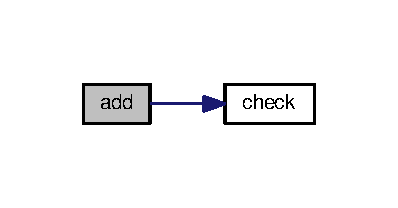
\includegraphics[width=191pt]{HiTester_8cpp_ab1aa54e6e8c6afe839f1b2e1456634b0_cgraph}
\end{center}
\end{figure}


\index{Hi\+Tester.\+cpp@{Hi\+Tester.\+cpp}!check@{check}}
\index{check@{check}!Hi\+Tester.\+cpp@{Hi\+Tester.\+cpp}}
\subsubsection[{\texorpdfstring{check(vector$<$ int $>$ v)}{check(vector< int > v)}}]{\setlength{\rightskip}{0pt plus 5cm}bool check (
\begin{DoxyParamCaption}
\item[{vector$<$ int $>$}]{v}
\end{DoxyParamCaption}
)}\hypertarget{HiTester_8cpp_a50e1d1eacaf36a74c01e52a2d1dd9ecd}{}\label{HiTester_8cpp_a50e1d1eacaf36a74c01e52a2d1dd9ecd}

\begin{DoxyCode}
141 \{
142    \textcolor{keywordflow}{if}(v.size() < 40)
143       \textcolor{keywordflow}{return} \textcolor{keyword}{true};
144    \textcolor{keywordflow}{else}
145       \textcolor{keywordflow}{return} \textcolor{keyword}{false};
146 \}
\end{DoxyCode}
\index{Hi\+Tester.\+cpp@{Hi\+Tester.\+cpp}!equal\+To@{equal\+To}}
\index{equal\+To@{equal\+To}!Hi\+Tester.\+cpp@{Hi\+Tester.\+cpp}}
\subsubsection[{\texorpdfstring{equal\+To(vector$<$ int $>$ v1, vector$<$ int $>$ v2)}{equalTo(vector< int > v1, vector< int > v2)}}]{\setlength{\rightskip}{0pt plus 5cm}bool equal\+To (
\begin{DoxyParamCaption}
\item[{vector$<$ int $>$}]{v1, }
\item[{vector$<$ int $>$}]{v2}
\end{DoxyParamCaption}
)}\hypertarget{HiTester_8cpp_ade6e4a501f91be609ebec2ff4f53f177}{}\label{HiTester_8cpp_ade6e4a501f91be609ebec2ff4f53f177}

\begin{DoxyCode}
149 \{
150    \textcolor{keywordflow}{if}(v1.size() != v2.size())
151       \textcolor{keywordflow}{return} \textcolor{keyword}{false};
152    \textcolor{keywordflow}{else}
153    \{
154       \textcolor{keywordtype}{int} count = 0;
155       \textcolor{keywordflow}{for}(\textcolor{keywordtype}{int} k=0; k<v1.size(); k++)
156       \{
157          \textcolor{keywordflow}{if}(v1[k] == v2[k])
158             count++;
159       \}
160       \textcolor{keywordflow}{if}(count == v1.size())
161          \textcolor{keywordflow}{return} \textcolor{keyword}{true};
162       \textcolor{keywordflow}{else}
163          \textcolor{keywordflow}{return} \textcolor{keyword}{false};
164    \}
165 \}
\end{DoxyCode}
\index{Hi\+Tester.\+cpp@{Hi\+Tester.\+cpp}!greater\+Than\+Or\+Equal@{greater\+Than\+Or\+Equal}}
\index{greater\+Than\+Or\+Equal@{greater\+Than\+Or\+Equal}!Hi\+Tester.\+cpp@{Hi\+Tester.\+cpp}}
\subsubsection[{\texorpdfstring{greater\+Than\+Or\+Equal(vector$<$ int $>$ v1, vector$<$ int $>$ v2)}{greaterThanOrEqual(vector< int > v1, vector< int > v2)}}]{\setlength{\rightskip}{0pt plus 5cm}bool greater\+Than\+Or\+Equal (
\begin{DoxyParamCaption}
\item[{vector$<$ int $>$}]{v1, }
\item[{vector$<$ int $>$}]{v2}
\end{DoxyParamCaption}
)}\hypertarget{HiTester_8cpp_a9a5f44b0a0b7a897f035c1137b066e16}{}\label{HiTester_8cpp_a9a5f44b0a0b7a897f035c1137b066e16}

\begin{DoxyCode}
183 \{
184    \textcolor{keywordflow}{if}(v1.size() > v2.size())
185       \textcolor{keywordflow}{return} \textcolor{keyword}{true};
186    \textcolor{keywordflow}{else} \textcolor{keywordflow}{if}(v1.size() < v2.size())
187       \textcolor{keywordflow}{return} \textcolor{keyword}{false};
188    \textcolor{keywordflow}{else}
189    \{
190       \textcolor{keywordflow}{for}(\textcolor{keywordtype}{int} k=0; k<v1.size(); k++)
191       \{
192          \textcolor{keywordflow}{if}(v1[k] > v2[k])
193             \textcolor{keywordflow}{return} \textcolor{keyword}{true};
194          \textcolor{keywordflow}{if}(v1[k] < v2[k])
195             \textcolor{keywordflow}{return} \textcolor{keyword}{false};
196       \}
197       \textcolor{keywordflow}{return} \textcolor{keyword}{true};
198    \}
199 \}
\end{DoxyCode}
\index{Hi\+Tester.\+cpp@{Hi\+Tester.\+cpp}!less\+Than\+Or\+Equal@{less\+Than\+Or\+Equal}}
\index{less\+Than\+Or\+Equal@{less\+Than\+Or\+Equal}!Hi\+Tester.\+cpp@{Hi\+Tester.\+cpp}}
\subsubsection[{\texorpdfstring{less\+Than\+Or\+Equal(vector$<$ int $>$ v1, vector$<$ int $>$ v2)}{lessThanOrEqual(vector< int > v1, vector< int > v2)}}]{\setlength{\rightskip}{0pt plus 5cm}bool less\+Than\+Or\+Equal (
\begin{DoxyParamCaption}
\item[{vector$<$ int $>$}]{v1, }
\item[{vector$<$ int $>$}]{v2}
\end{DoxyParamCaption}
)}\hypertarget{HiTester_8cpp_a39022c885b9928f13a6c4987dc563b60}{}\label{HiTester_8cpp_a39022c885b9928f13a6c4987dc563b60}

\begin{DoxyCode}
202 \{
203    \textcolor{keywordflow}{if}(v1.size() < v2.size())
204       \textcolor{keywordflow}{return} \textcolor{keyword}{true};
205    \textcolor{keywordflow}{else} \textcolor{keywordflow}{if}(v1.size() > v2.size())
206       \textcolor{keywordflow}{return} \textcolor{keyword}{false};
207    \textcolor{keywordflow}{else}
208    \{
209       \textcolor{keywordflow}{for}(\textcolor{keywordtype}{int} k=0; k<v1.size(); k++)
210       \{
211          \textcolor{keywordflow}{if}(v1[k] < v2[k])
212             \textcolor{keywordflow}{return} \textcolor{keyword}{true};
213          \textcolor{keywordflow}{if}(v1[k] > v2[k])
214             \textcolor{keywordflow}{return} \textcolor{keyword}{false};
215       \}
216       \textcolor{keywordflow}{return} \textcolor{keyword}{true};
217    \}
218 
219 \}
\end{DoxyCode}
\index{Hi\+Tester.\+cpp@{Hi\+Tester.\+cpp}!main@{main}}
\index{main@{main}!Hi\+Tester.\+cpp@{Hi\+Tester.\+cpp}}
\subsubsection[{\texorpdfstring{main()}{main()}}]{\setlength{\rightskip}{0pt plus 5cm}int main (
\begin{DoxyParamCaption}
{}
\end{DoxyParamCaption}
)}\hypertarget{HiTester_8cpp_ae66f6b31b5ad750f1fe042a706a4e3d4}{}\label{HiTester_8cpp_ae66f6b31b5ad750f1fe042a706a4e3d4}

\begin{DoxyCode}
17 \{
18    \textcolor{keywordtype}{int} a, b;
19    \textcolor{keywordtype}{char} c;
20    cout << \textcolor{stringliteral}{"enter equation: "};
21    cin >> a >> c >> b;
22    cout << a << \textcolor{stringliteral}{" "} << c << \textcolor{stringliteral}{" "} << b << endl;
23 
24    vector<int> v;                                                                                          
                                                                                                       
25    \textcolor{keywordtype}{int} array1[7] = \{1, 9, 5, 3, 6, 0, 0\};                                                                  
                                                                                                       
26    \textcolor{keywordtype}{int} len1 = 5;                                                                                           
                                                                                                       
27    \textcolor{keywordtype}{int} array2[7] = \{4, 8, 2, 2, 0, 1, 3\};                                                                  
                                                                                                       
28    \textcolor{keywordtype}{int} len2 = 7;                                                                                           
                                                                                                       
29    v = \hyperlink{HiTester_8cpp_ab1aa54e6e8c6afe839f1b2e1456634b0}{add}(array1, array2, len1, len2);                                                                 
                                                                                                          
30    \textcolor{keywordflow}{for}(\textcolor{keywordtype}{int} k=0; k<v.size(); k++)                                                                           
                                                                                                       
31       cout << v[k] << \textcolor{stringliteral}{" "};                                                                                 
                                                                                                       
32    cout << endl;                                                                                           
                                                                                                       
33                                                                                                            
                                                                                                       
34    \textcolor{keywordtype}{int} a1[8] = \{1, 3, 7, 2, 0, 7, 7, 8\};                                                                   
                                                                                                       
35    \textcolor{keywordtype}{int} a2[8] = \{7, 3, 4, 0, 0, 0, 0, 0\};                                                                   
                                                                                                       
36    len1 = 8;                                                                                               
                                                                                                       
37    len2 = 3;                                                                                               
                                                                                                       
38    v = \hyperlink{HiTester_8cpp_ab1aa54e6e8c6afe839f1b2e1456634b0}{add}(a1, a2, len1, len2);                                                                         
                                                                                                          
39    \textcolor{keywordflow}{for}(\textcolor{keywordtype}{int} k=0; k<v.size(); k++)                                                                           
                                                                                                       
40       cout << v[k] << \textcolor{stringliteral}{" "};                                                                                 
                                                                                                       
41    cout << endl << endl;                                                                                   
                                                                                                       
42                                                                                                            
                                                                                                       
43    \hyperlink{HiTester_8cpp_ab1aa54e6e8c6afe839f1b2e1456634b0}{add}(array1, array2);                                                                                 
                                                                                                          
44    cout << endl;                                                                                           
                                                                                                       
45    \hyperlink{HiTester_8cpp_ab1aa54e6e8c6afe839f1b2e1456634b0}{add}(a1, a2);                                                                                         
                                                                                                          
46    cout << endl;                                                                                           
                                                                                                       
47                                                                                                            
                                                                                                       
48    vector<int> num1, num2;                                                                                 
                                                                                                       
49    \textcolor{keywordflow}{for}(\textcolor{keywordtype}{int} k=0; k<7; k++)                                                                                  
                                                                                                       
50       num1.push\_back(k);                                                                                   
                                                                                                       
51    \textcolor{keywordflow}{for}(\textcolor{keywordtype}{int} j=3; j>=0; j--)                                                                                 
                                                                                                       
52       num2.push\_back(j);                                                                                   
                                                                                                       
53                                                                                                            
                                                                                                       
54    \textcolor{keywordflow}{if}(\hyperlink{HiTester_8cpp_ade6e4a501f91be609ebec2ff4f53f177}{equalTo}(num1, num2))                                                                          
                                                                                                              
55       cout << \textcolor{stringliteral}{"EQUAL!!"} << endl;                                                                           
                                                                                                       
56    \textcolor{keywordflow}{else}                                                                                                    
                                                                                                       
57       cout << \textcolor{stringliteral}{"NOT EQUAL!!!"} << endl;                                                                      
                                                                                                       
58                                                                                                            
                                                                                                       
59    \textcolor{keywordflow}{if}(\hyperlink{HiTester_8cpp_ade6e4a501f91be609ebec2ff4f53f177}{equalTo}(num1, num1))
60       cout << \textcolor{stringliteral}{"EQUAL!!!"} << endl;                                                                          
                                                                                                       
61    \textcolor{keywordflow}{else}                                                                                                    
                                                                                                       
62       cout << \textcolor{stringliteral}{"NOT EQUAL!!"} << endl;                                                                       
                                                                                                       
63                                                                                                            
                                                                                                       
64    \textcolor{keywordflow}{if}(\hyperlink{HiTester_8cpp_a4c5b23015a428515b186958f049fa9ff}{notEqual}(num1, num2))                                                                        
                                                                                                               
65       cout << \textcolor{stringliteral}{"NOT EQUAL!!"} << endl;                                                                       
                                                                                                       
66    \textcolor{keywordflow}{else}                                                                                                    
                                                                                                       
67       cout << \textcolor{stringliteral}{"EQUAL!!!"} << endl;                                                                          
                                                                                                       
68                                                                                                            
                                                                                                       
69    \textcolor{keywordflow}{if}(\hyperlink{HiTester_8cpp_a4c5b23015a428515b186958f049fa9ff}{notEqual}(num1, num1))                                                                        
                                                                                                               
70       cout << \textcolor{stringliteral}{"NOT EQUAL!!!"} << endl;                                                                      
                                                                                                       
71    \textcolor{keywordflow}{else}                                                                                                    
                                                                                                       
72       cout << \textcolor{stringliteral}{"EQUAL!!"} << endl;                                                                           
                                                                                                       
73                                                                                                            
                                                                                                       
74    \textcolor{keywordflow}{if}(\hyperlink{HiTester_8cpp_a9a5f44b0a0b7a897f035c1137b066e16}{greaterThanOrEqual}(num1, num2))                                                    
                                                                                                                  
             
75       cout << \textcolor{stringliteral}{"Greater Than Or Equal To!!"} << endl;                                                        
                                                                                                       
76    \textcolor{keywordflow}{else}                                                                                                    
                                                                                                       
77       cout << \textcolor{stringliteral}{"Less Than!!!"} << endl;                                                                      
                                                                                                       
78                                                                                                            
                                                                                                       
79    \textcolor{keywordflow}{if}(\hyperlink{HiTester_8cpp_a9a5f44b0a0b7a897f035c1137b066e16}{greaterThanOrEqual}(num1, num1))                                                    
                                                                                                                  
             
80       cout << \textcolor{stringliteral}{"Greater than or Equal to!!!"} << endl;                                                       
                                                                                                       
81    \textcolor{keywordflow}{else}                                                                                                    
                                                                                                       
82       cout << \textcolor{stringliteral}{"Less Than!!"} << endl;                                                                       
                                                                                                       
83                                                                                                            
                                                                                                       
84    \textcolor{keywordflow}{if}(\hyperlink{HiTester_8cpp_a9a5f44b0a0b7a897f035c1137b066e16}{greaterThanOrEqual}(num2, num1))                                                    
                                                                                                                  
             
85       cout << \textcolor{stringliteral}{"Greater than or Equal to!!!"} << endl;                                                       
                                                                                                       
86    \textcolor{keywordflow}{else}                                                                                                    
                                                                                                       
87       cout << \textcolor{stringliteral}{"Less Than!!"} << endl;                                                                       
                                                                                                       
88                                                                                                            
                                                                                                       
89    \textcolor{keywordflow}{if}(\hyperlink{HiTester_8cpp_a39022c885b9928f13a6c4987dc563b60}{lessThanOrEqual}(num1, num2))
90       cout << \textcolor{stringliteral}{"Less Than Or Equal To!!"} << endl;                                                           
                                                                                                       
91    \textcolor{keywordflow}{else}                                                                                                    
                                                                                                       
92       cout << \textcolor{stringliteral}{"Greater Than!!!"} << endl;                                                                   
                                                                                                       
93                                                                                                            
                                                                                                       
94    \textcolor{keywordflow}{if}(\hyperlink{HiTester_8cpp_a39022c885b9928f13a6c4987dc563b60}{lessThanOrEqual}(num1, num1))                                                          
                                                                                                                  
          
95       cout << \textcolor{stringliteral}{"Less than or Equal to!!!"} << endl;                                                          
                                                                                                       
96    \textcolor{keywordflow}{else}                                                                                                    
                                                                                                       
97       cout << \textcolor{stringliteral}{"Greater Than!!"} << endl;                                                                    
                                                                                                       
98                                                                                                            
                                                                                                       
99    \textcolor{keywordflow}{if}(\hyperlink{HiTester_8cpp_a39022c885b9928f13a6c4987dc563b60}{lessThanOrEqual}(num2, num1))                                                          
                                                                                                                  
          
100       cout << \textcolor{stringliteral}{"Less than or Equal to!!!"} << endl;                                                          
                                                                                                       
101    \textcolor{keywordflow}{else}                                                                                                    
                                                                                                       
102       cout << \textcolor{stringliteral}{"Greater Than!!"} << endl;                                                                    
                                                                                                       
103 
104    \textcolor{keywordflow}{return} 0;
105 \}
\end{DoxyCode}


Here is the call graph for this function\+:
\nopagebreak
\begin{figure}[H]
\begin{center}
\leavevmode
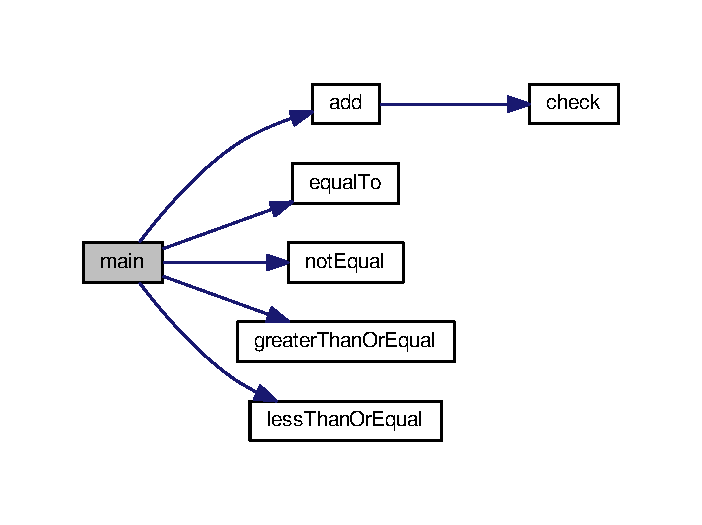
\includegraphics[width=337pt]{HiTester_8cpp_ae66f6b31b5ad750f1fe042a706a4e3d4_cgraph}
\end{center}
\end{figure}


\index{Hi\+Tester.\+cpp@{Hi\+Tester.\+cpp}!not\+Equal@{not\+Equal}}
\index{not\+Equal@{not\+Equal}!Hi\+Tester.\+cpp@{Hi\+Tester.\+cpp}}
\subsubsection[{\texorpdfstring{not\+Equal(vector$<$ int $>$ v1, vector$<$ int $>$ v2)}{notEqual(vector< int > v1, vector< int > v2)}}]{\setlength{\rightskip}{0pt plus 5cm}bool not\+Equal (
\begin{DoxyParamCaption}
\item[{vector$<$ int $>$}]{v1, }
\item[{vector$<$ int $>$}]{v2}
\end{DoxyParamCaption}
)}\hypertarget{HiTester_8cpp_a4c5b23015a428515b186958f049fa9ff}{}\label{HiTester_8cpp_a4c5b23015a428515b186958f049fa9ff}

\begin{DoxyCode}
168 \{
169    \textcolor{keywordflow}{if}(v1.size() != v2.size())
170       \textcolor{keywordflow}{return} \textcolor{keyword}{true};
171    \textcolor{keywordflow}{else}
172    \{
173       \textcolor{keywordflow}{for}(\textcolor{keywordtype}{int} k=0; k<v1.size(); k++)
174       \{
175          \textcolor{keywordflow}{if}(v1[k] != v2[k])
176             \textcolor{keywordflow}{return} \textcolor{keyword}{true};
177       \}
178       \textcolor{keywordflow}{return} \textcolor{keyword}{false};
179    \}
180 \}
\end{DoxyCode}

%--- End generated contents ---

% Index
\backmatter
\newpage
\phantomsection
\clearemptydoublepage
\addcontentsline{toc}{chapter}{Index}
\printindex

\end{document}
